% -*- coding: UTF-8 -*-
% vim: autoindent expandtab tabstop=4 sw=4 sts=4 filetype=tex
% vim: spelllang=de spell
% chktex-file 27 - disable warning about missing include files

\section{Sequenz-Diagramme}
\label{sec:sequence-diagrams}

Gemäss~\cite{larman_applying_2004} stellen Sequenz-Diagramme Ereignisse, welche
externe Akteure auslösen bzw.\ generieren, deren Ablauf sowie Ereignisse
zwischen Systemen eines spezifischen Szenarios eines Use Cases dar.

Da Sequenz-Diagramme schnell eine gewisse Grösse und auch Komplexität annehmen
wird in dieser Projektarbeit darauf verzichtet ein Sequenz-Diagramm für alle
Use Cases zu erstellen. Gerade bei \```UC2: Erstellen einer
Echtzeit-Animation\''' würde dies ansonsten grosse Ausmasse annehmen. Bei
Bedarf können diese bei den einzelnen Iterationen bzw.\ Phasen (Elaboration,
Construction und Transition). An dieser Stelle wird daher nur das
Sequenz-Diagramm für den ersten Use Case, \```UC1: Betrachten einer
Echtzeit-Animation\''' dargestellt. Dies deckt bereits einen Teil des Editors
mit ab.

\begin{figure}[H]
    \centering
    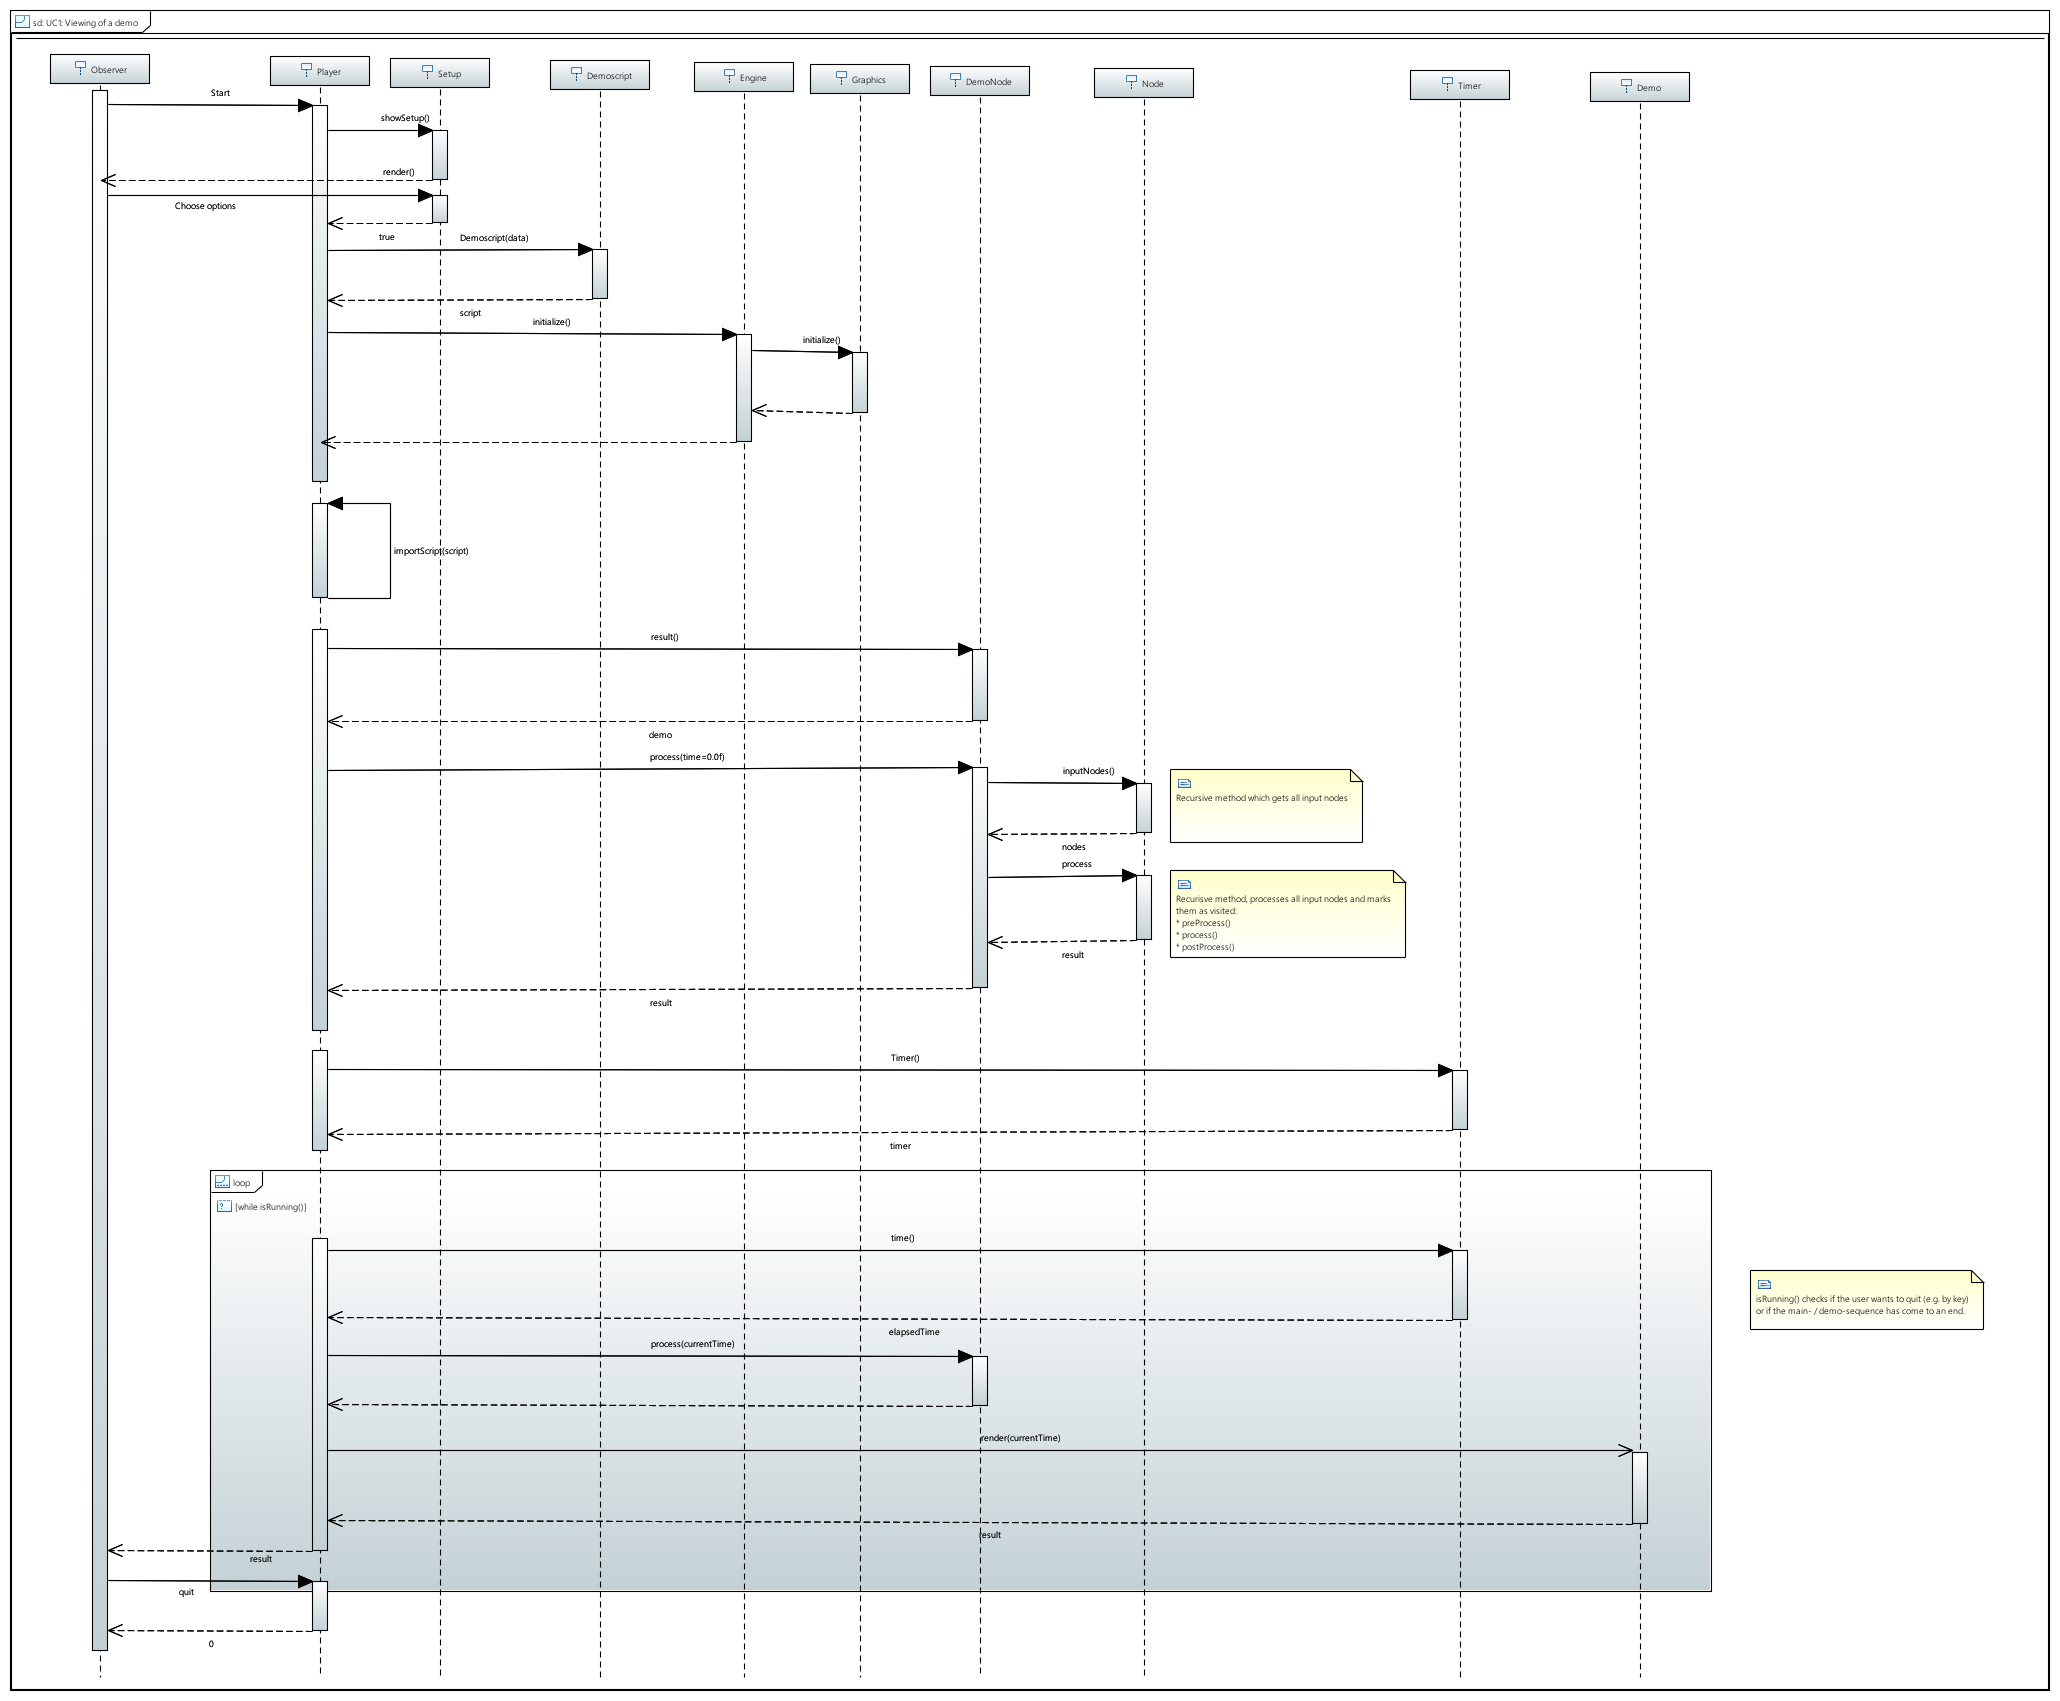
\includegraphics[angle=90,width=0.9\textwidth]{img/sequence_diagram_uc1.pdf}
    \caption{Sequenz-Diagramm  des Use Cases UC1
        \protect\footnotemark}\label{fig:package-diagram:editor}
\end{figure}
\footnotetext{Eigene Darstellung mittels Papyrus.}

\todo[inline]{Describe sequence diagram.}
